
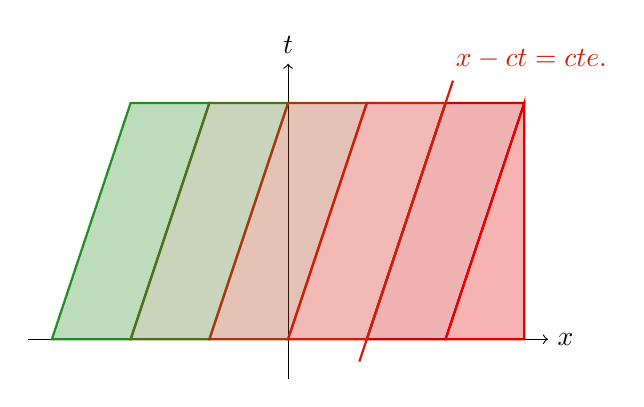
\begin{tikzpicture}

\draw[->] (-3.3, 0) -- (3.3,0) node[right] {$x$};
\draw[->] (0, -0.5) -- (0,3.5) node[above] {$t$};

\draw[thick, ForestGreen, fill opacity = 0.3, fill = ForestGreen]
	(-3, 0) -- (-2, 0) -- (-1, 3) -- (-2, 3) -- cycle;
\draw[thick, ForestGreen!80!red, fill opacity = 0.3, fill = ForestGreen!80!red]
	(-2, 0) -- (-1, 0) -- (0, 3) -- (-1, 3) -- cycle;
\draw[thick, ForestGreen!40!red, fill opacity = 0.3, fill = ForestGreen!40!red]
	(-1, 0) -- (0, 0) -- (1,3) -- (0,3) -- cycle;
\draw[thick, ForestGreen!20!red, fill opacity = 0.3, fill = ForestGreen!20!red]
	(0, 0) -- (1, 0) -- (2,3) -- (1,3) -- cycle;
\draw[thick, red!80!black, fill opacity = 0.3, fill = red!80!black]
	(1, 0) -- (2, 0) -- (3,3) -- (2,3) -- cycle;
\draw[thick, red!90!black, fill opacity = 0.3, fill = red!90!black]
	(2, 0) -- (3, 0) -- (3,3) -- cycle;

\draw[thick, ForestGreen!20!red, shorten >= -0.3cm, shorten <= -0.3cm]
	(1, 0) -- (2,3) node[anchor = south west, yshift = 0.3cm] {$x - ct = \text{cte.}$};


\end{tikzpicture}
